\documentclass{./../../Latex/teaching_slides}

\usepackage{venndiagram}
\usepackage{tikz}
\usepackage{pgfplots}
\usetikzlibrary{arrows.meta}

\begin{document}

\title{ECON 441 \\ \vspace{0.4em} \normalsize Introduction to Mathematical Economics}
\author{Div Bhagia}
\date{Lecture 8: Unconstrained Single Variable Optimization, \\ Concave \& Convex Functions}

%%%%%%%%%%%%%%
\begin{frame}[noframenumbering, plain]
\maketitle
\end{frame}

%%%%%%%%%%%%%%
\begin{frame}{Optimization}
How many hours to work each week? \\~\\
Utility from consumption ($C$) and leisure ($L$):
$$ U(C,L) $$
Leisure is the difference between total hours ($T$) and hours worked ($H$)
$$L = T-H$$
Constraint:
$$ wH = pC $$
where $w$ and $p$ denote wages and price, respectively.
\end{frame}

%%%%%%%%%%%%%%
\begin{frame}{Global vs Local Extrema}
\centering
\includegraphics[scale=0.375]{global_vs_local.png}
\end{frame}

%%%%%%%%%%%%%%
\begin{frame}{Critical Points}
Limit ourselves to functions that are \textit{continuously differentiable} i.e. $f$ is continuous and has a continuous derivative. 
$$ y = f(x) $$ 

A \textit{necessary} condition for $x_0$ to be an extremum \\
$$f'(x_0) = 0$$ 

$x_0$ is called a critical/stationary point. \\~\\
Why not sufficient?
\end{frame}

%%%%%%%%%%%%%%
\begin{frame}{Inflection Point}
\centering
\includegraphics[scale=0.5]{inflection.png}
\end{frame}

%%%%%%%%%%%%%%
\begin{frame}{First-Derivative Test}
Suppose that $f^{\prime}\left(x_{0}\right)=0$. Then $f\left(x_{0}\right)$ is a \\~\\

\begin{enumerate}
  \item maximum if $f^{\prime}(x)$ goes from $+$ to $-$ in the immediate neighborhood of $x_{0}$ \\~\\
  \item minimum if $f^{\prime}(x)$ goes from $-$ to $+$ in the immediate neighborhood of $x_{0}$ \\~\\

  \item not an extreme point if $f^{\prime}(x)$ has the same sign in its immediate neighborhood
\end{enumerate}
\end{frame}

%%%%%%%%%%%%%%
\begin{frame}{First-Derivative Test}
\centering
\begin{tikzpicture}[scale=1.25, transform shape]
\begin{axis}[axis lines = center, ymax=3, xtick, ytick, ymin=-2, xmin=-35, xmax=65]
\addplot [domain=-30:60, samples=100, line width = 0.3mm]
{cos(5*x+2)+cos(2*x+2)};
\draw[dashed,red] (250,400) -- (450,400) node[above, yshift=-2, xshift=0] {\scriptsize $f'(x)=0$};
\draw[dashed,red] (650,120) -- (850,120)node[above, yshift=-20, xshift=-12] {\scriptsize $f'(x)=0$};
\node[right, rotate=-60, red] at (480,370) {\scriptsize $f'(x)<0$};
\node[right, rotate=60, red] at (100,255) {\scriptsize $f'(x)>0$};
\node[right, rotate=-30, red] at (480,200) {\scriptsize $f'(x)<0$};
\node[right, rotate=30, red] at (825,120) {\scriptsize $f'(x)>0$};
\end{axis}

    % Axes
    %\draw[->] (-4,0) -- (4,0) node[right] {$x$};
    %\draw[->] (0,-2) -- (0,4) node[above] {$y$};
    % Function f(x)
    %\draw[domain=-3:3,smooth,variable=\x,blue] plot ({\x},{0.2*\x^3+0.1*\x^2-0.5*\x});
    % Tangent lines
    %\draw[dashed,red] (-2.5,-0.375) -- (2.5,1.125);
    %\draw[dashed,red] (-1.2,-0.24) -- (1.2,0.24);
    % Intersection points
    %\draw[fill=white] (-2.14,-0.257) circle [radius=2pt] node[below left] {$(x_1, f(x_1))$};
    %\draw[fill=white] (2.14,0.257) circle [radius=2pt] node[above right] {$(x_2, f(x_2))$};
    %\draw[fill=white] (-0.4,-0.32) circle [radius=2pt] node[below left] {$(\bar{x}, \bar{y})$};
    % Vertical lines
    %\draw[dashed] (-2.14,0) -- (-2.14,-0.257);
    %\draw[dashed] (2.14,0) -- (2.14,0.257);
    %\draw[dashed] (-0.4,0) -- (-0.4,-0.32);
    % Labels
    %\node[below] at (-2.14,0) {$x_1$};
    %\node[below] at (2.14,0) {$x_2$};
    %\node[below] at (-0.4,0) {$\bar{x}$};
    %\node[left] at (0,-0.5) {$f'(\bar{x}) = 0$};
    %\node[right] at (2.5,1.125) {$y = f'(x_1)x + f(x_1)$};
    %\node[right] at (1.2,0.24) {$y = f'(\bar{x})x + \bar{y}$};
\end{tikzpicture}
\end{frame}



%%%%%%%%%%%%%%
\begin{frame}{Example}
Let's find the extrema for the following function:
$$ f(x) = x^2-24x+36 $$
%\begin{tikzpicture}[scale=0.75, transform shape]
%\begin{axis}[axis lines = center, xlabel = \(x\), ylabel = \(f(x)\), xmin=-5, xmax=27]
%\addplot [domain=0:25, samples=100, color=red, line width = 0.5mm]
%{x^2-24*x+36};
%\end{axis}
%\end{tikzpicture}
\end{frame}

%%%%%%%%%%%%%%
\begin{frame}{Example}
Total cost: $$ TC = C(Q)$$
Marginal cost: $$ MC = C'(Q) $$
Average cost: $$ AC = \frac{C(Q)}{Q} $$ \\~\\
At what quantity is $AC$ the lowest? 
\end{frame}

%%%%%%%%%%%%%%
\begin{frame}{Average and Marginal Cost}
\centering
\includegraphics[scale=0.7]{AC-MC.jpg}
\end{frame}

%%%%%%%%%%%%%%
\begin{frame}{Second and Higher Derivatives}
The derivative of $f^{\prime}(x)$ is called the second derivative and is denoted by:
$$ f^{\prime \prime}(x) = \frac{d^{2} y }{ d x^{2}}$$
Similarly, we can obtain other higher-order derivatives:
$$
f^{3}(x), f^{(4)}(x), \cdots, f^{(n)}(x)
$$
or
$$
\frac{d^{3} y}{d x^{3}}, \frac{d^{4} y}{d x^{4}}, \cdots, \frac{d^{n} y}{d x^{n}}
$$
\end{frame}

%%%%%%%%%%%%%%
\begin{frame}{Second Derivative}
With an infinitesimal increase in $x$ from $x_0$ \\~\\

\begin{witemize}
  \item \textit{Value} of the function increases if $f'(x_0)>0$
  \item \textit{Value} of the function decreases if $f'(x_0)<0$ \\~\\
  \item \textit{Slope} of the function increases if $f''(x_0)>0$
  \item \textit{Slope} of the function decreases if $f''(x_0)<0$
\end{witemize}
\end{frame}

%%%%%%%%%%%%%%
\begin{frame}{Second Derivative Test}
If $f^{\prime}\left(x_{0}\right)=0$, then the value of the function at $x_{0}, f\left(x_{0}\right)$ will be \\~\\
\begin{enumerate}
  \item a maximum if $f''(x_0)<0$
  \item a minimum if $f''(x_0)>0$ \\~\\
\end{enumerate}
More convenient to use than the first-derivative test.
\end{frame}

%%%%%%%%%%%%%%
\begin{frame}{Necessary vs Sufficient Conds.}
\begin{tabularx}{\textwidth}{lXX}
\hline Condition & Maximum & Minimum \\
\hline \\ 
First-order necessary & $f^{\prime}(x)=0$ & $f^{\prime}(x)=0$ \\~\\
Second-order necessary ${ }^{\dagger}$ & $f^{\prime \prime}(x) \leq 0$ & $f^{\prime \prime}(x) \geq 0$ \\~\\
Second-order sufficient ${ }^{\dagger}$ & $f^{\prime \prime}(x)<0$ & $f^{\prime \prime}(x)>0$ \\~\\
\hline
\end{tabularx}
\vspace{0.25em}

${ }^{\dagger}$ Applicable only after the first-order necessary condition has been satisfied.
\end{frame}

%%%%%%%%%%%%%%
\begin{frame}{Necessary vs Sufficient Conds.}
\vspace{-1.5em}
$$ y = x^4 $$ \\~\\
\centering
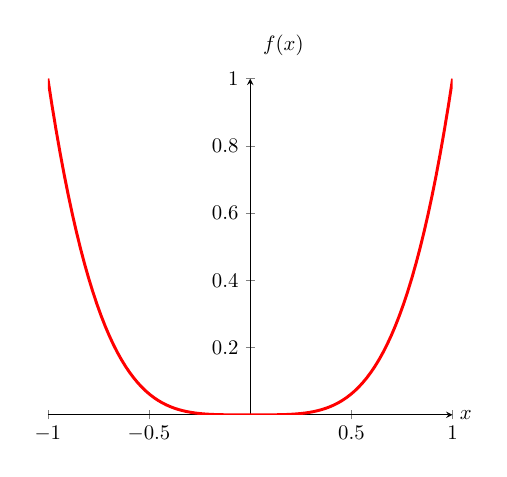
\begin{tikzpicture}[scale=0.75, transform shape]
\begin{axis}[axis lines = center, xlabel = \(x\), ylabel = \(f(x)\),
  xlabel style={at={(axis description cs:1,0)}, anchor=west},
  ylabel style={at={(axis description cs:0.65,1.1)}, anchor=east}
]
\addplot [domain=-1:1, samples=100, color=red, line width = 0.5mm]
{x^4};
\end{axis}
\end{tikzpicture}
\end{frame}

%%%%%%%%%%%%%%
\begin{frame}{Concave and Convex Functions}
\begin{witemize}
  \item Concave function: $ f''(x) \leq 0$ for all $x$ 
  \item Convex function: $ f''(x) \geq 0$ for all $x$ \\~\\
  \item Strictly concave function: $ f''(x) < 0$ for all $x$ 
  \item Strictly convex function: $ f''(x) > 0$ for all $x$ 
\end{witemize}
\end{frame}

%%%%%%%%%%%%%%
\begin{frame}{Concave and Convex Functions}
$f$ is concave if:
$$ f(\lambda x_1 + (1-\lambda) x_2) \geq \lambda f(x_1) + (1-\lambda) f(x_2)  $$
$f$ is covex if:
$$ f(\lambda x_1 + (1-\lambda) x_2) \leq \lambda f(x_1) + (1-\lambda) f(x_2)  $$
where $\lambda \in (0,1)$.\\
\vspace{1em}
For strict concavity/convexity replace with strict inequalities. 
\end{frame}

\pgfmathdeclarefunction{func}{1}{%
  \pgfmathparse{5*(#1)^0.4-2*(#1)^3-2}%
}
%%%%%%%%%%%%%%
\begin{frame}{Concave Function}
\begin{tikzpicture}[scale=1.25, transform shape]
\begin{axis}[axis lines = center, ytick distance=100, xtick distance=100, extra x ticks = {}, ymin=-0, ymax=1.75, xmin=-0.3, xmax=0.75, enlarge x limits=0.15, enlarge y limits=0.15, width=12cm, height=7.75cm]
\addplot [domain=0.1:1, samples=100, color=red, line width = 0.4mm]
{func(x)};
% Two points: xaxis
\node[circle,fill,inner sep=1pt, label=below:{\footnotesize $x_1$}] at (axis cs:0.2,0) {};
\node[circle,fill,inner sep=1pt, label=below:{\footnotesize $x_2$}] at (axis cs:0.7,0) {};
% Two points: yaxis
\node[circle,fill,inner sep=1pt] at (axis cs:0.2,{func(0.2)}) {};
\node[circle,fill,inner sep=1pt] at (axis cs:0.7,{func(0.7)}) {};
% Two vertical lines
\draw[dashed] (axis cs:0.2,0) -- (axis cs:0.2,{func(0.2)});
\draw[dashed] (axis cs:0.7,0) -- (axis cs:0.7,{func(0.7)});
% Two Horizontal lines
\draw[dashed] (axis cs:0.2,{func(0.2)}) -- (axis cs:0,{func(0.2)});
\draw[dashed] (axis cs:0.7,{func(0.7)}) -- (axis cs:0,{func(0.7)});
% Tangent line
\draw[dashed] (axis cs:0.2,{func(0.2)}) -- (axis cs:0.7,{func(0.7)});
% Linear combination of x1 & x2
\node[circle,fill,inner sep=1pt] at (axis cs:0.45,{func(0.45)}) {};
\node[circle,fill,inner sep=1pt, label=below:{\footnotesize $\lambda x_1 + (1-\lambda)x_2$}] at (axis cs:0.45,0) {};
\draw[dashed] (axis cs:0.45,0) -- (axis cs:0.45,{func(0.45)});
\draw[dashed] (axis cs:0.45,{func(0.45)}) -- (axis cs:0,{func(0.45)});
% Linear combination of fx1 & fx2
\node[circle,fill,inner sep=1pt] at (axis cs:0.45,{0.5*func(0.7)+0.5*func(0.2)}) {};
\draw[dashed] (axis cs:0.45,{0.5*func(0.7)+0.5*func(0.2)}) -- (axis cs:0,{0.5*func(0.7)+0.5*func(0.2)});
% Markers on the yaxis
\node[circle,fill,inner sep=1pt, label=left:{\footnotesize $f(x_2)$}] at (axis cs:0,{func(0.7)}) {};
\node[circle,fill,inner sep=1pt, label=left:{\footnotesize $f(x_1)$}] at (axis cs:0,{func(0.2)}) {};
\node[circle,fill,inner sep=1pt, label=left:{\footnotesize $\lambda f(x_1) + (1-\lambda)f(x_2)$}] at (axis cs:0,{0.5*func(0.7)+0.5*func(0.2)}) {};
\node[circle,fill,inner sep=1pt, label=left:{\footnotesize $f(\lambda x_1 + (1-\lambda)x_2)$}] at (axis cs:0,{func(0.45)}) {};
\end{axis}
\end{tikzpicture}
\end{frame}

\pgfmathdeclarefunction{funco}{1}{%
  \pgfmathparse{4*(#1)^3+(#1)^2-1*(#1)^1+0.5}%
}
%%%%%%%%%%%%%%
\begin{frame}{Convex Function}
\begin{tikzpicture}[scale=1.25, transform shape]
\begin{axis}[axis lines = center, ytick distance=100, xtick distance=100, extra x ticks = {}, ymin=-0, ymax=1.75, xmin=-0.3, xmax=0.75, enlarge x limits=0.15, enlarge y limits=0.15, width=12cm, height=7.75cm]
\addplot [domain=0.1:1, samples=100, color=red, line width = 0.4mm]
{funco(x)};
% Two points: xaxis
\node[circle,fill,inner sep=1pt, label=below:{\footnotesize $x_1$}] at (axis cs:0.2,0) {};
\node[circle,fill,inner sep=1pt, label=below:{\footnotesize $x_2$}] at (axis cs:0.7,0) {};
% Two points: yaxis
\node[circle,fill,inner sep=1pt] at (axis cs:0.2,{funco(0.2)}) {};
\node[circle,fill,inner sep=1pt] at (axis cs:0.7,{funco(0.7)}) {};
% Two vertical lines
\draw[dashed] (axis cs:0.2,0) -- (axis cs:0.2,{funco(0.2)});
\draw[dashed] (axis cs:0.7,0) -- (axis cs:0.7,{funco(0.7)});
% Two Horizontal lines
\draw[dashed] (axis cs:0.2,{funco(0.2)}) -- (axis cs:0,{funco(0.2)});
\draw[dashed] (axis cs:0.7,{funco(0.7)}) -- (axis cs:0,{funco(0.7)});
% Tangent line
\draw[dashed] (axis cs:0.2,{funco(0.2)}) -- (axis cs:0.7,{funco(0.7)});
% Linear combination of x1 & x2
\node[circle,fill,inner sep=1pt] at (axis cs:0.45,{funco(0.45)}) {};
\node[circle,fill,inner sep=1pt, label=below:{\footnotesize $\lambda x_1 + (1-\lambda)x_2$}] at (axis cs:0.45,0) {};
\draw[dashed] (axis cs:0.45,{funco(0.45)}) -- (axis cs:0,{funco(0.45)});
% Linear combination of fx1 & fx2
\node[circle,fill,inner sep=1pt] at (axis cs:0.45,{0.5*funco(0.7)+0.5*funco(0.2)}) {};
\draw[dashed] (axis cs:0.45,{0.5*funco(0.7)+0.5*funco(0.2)}) -- (axis cs:0,{0.5*funco(0.7)+0.5*funco(0.2)});
\draw[dashed] (axis cs:0.45,0) -- (axis cs:0.45,{0.5*funco(0.7)+0.5*funco(0.2)});
% Markers on the yaxis
\node[circle,fill,inner sep=1pt, label=left:{\footnotesize $f(x_2)$}] at (axis cs:0,{funco(0.7)}) {};
\node[circle,fill,inner sep=1pt, label=left:{\footnotesize $f(x_1)$}] at (axis cs:0,{funco(0.2)}) {};
\node[circle,fill,inner sep=1pt, label=left:{\footnotesize $\lambda f(x_1) + (1-\lambda)f(x_2$)}] at (axis cs:0,{0.5*funco(0.7)+0.5*funco(0.2)}) {};
\node[circle,fill,inner sep=1pt, label=left:{\footnotesize $f(\lambda x_1 + (1-\lambda)x_2)$}] at (axis cs:0,{funco(0.45)}) {};
\end{axis}
\end{tikzpicture}
\end{frame}


%%%%%%%%%%%%%%
\begin{frame}{Attitudes toward Risk}
Consider the following game: flip a coin, collect \$0 if tails, collect \$20 if heads. \\~\\
How much would you pay to play this game? 
\end{frame}

%%%%%%%%%%%%%%
\begin{frame}{Concave and Convex Functions}
The domain of $f$ is all real numbers
$$ f(x) = x^3 $$
Is $f$ a convex, strictly convex, concave, or strictly concave function? \\~\\
What if the domain of $f$ is all nonnegative real numbers? 
\end{frame}

%%%%%%%%%%%%%%
\begin{frame}{$f(x)=x^3$}
\begin{center}
\begin{tikzpicture}[scale=1.1, transform shape]
\begin{axis}[axis lines = center, xlabel = \(x\), ylabel = \(f(x)\), ytick distance=200, xtick distance=100, extra x ticks = {0}]
\addplot [domain=-0:5, samples=100, color=red, line width = 0.4mm]{x^3};
\addplot [domain=-5:5, samples=100, color=red, line width = 0.4mm, style=dashed]{x^3};
\end{axis}
\end{tikzpicture}
\end{center}
\end{frame}

\begin{frame}{Properties of Concave and Covex Functions}
1.  If $f(x)$ is a linear function, then it is a concave function as well as a convex function, but not strictly so. \\~\\

2. If $f(x)$ is a (strictly) concave function, then $-f(x)$ is a (strictly) convex function, and vice versa. \\~\\

3. If $f(x)$ and $g(x)$ are both concave (convex) functions, then $f(x)+g(x)$ is a concave (convex) function. Further, in addition, either one or both of them are strictly concave (strictly convex), then $f(x)+g(x)$ is strictly concave (convex).
\end{frame}

%%%%%%%%%%%%%%
\begin{frame}{Global Optimizers}
\begin{witemize}
  \item If a function is concave, any critical point will give us a global maximum.
  \item If a function is strictly concave, any critical point will give us the \textit{unique} global maximum.
  \item If a function is convex, any critical point will give us a global minimum.
  \item If a function is strictly convex, any critical point will give us the \textit{unique} global minimum.
\end{witemize}
\end{frame}


%%%%%%%%%%%%%%
\begin{frame}{Concave and Convex Functions}
Say, $f(x)$ is a strictly concave function and \\~\\
$$f'(2) = 0 $$ \\~\\
Is $f(2)$ the local or global maximum? Is it the unique maximum?
\end{frame}




%%%%%%%%%%%%%%
\begin{frame}{References and Homework}
\begin{witemize}
  \item Covered today: Sections 9.1, 9.2, 9.3, 9.4
  \item Homework problems: \\
  \begin{witemize}
  \normalsize
  \item Exercise 9.2: 1 (c), 2 (a), 3, 4
  \item Exercise 9.3: 2, 3, 4, 5 
  \item Exercise 9.4: 1 (b) (d), 2, 3, 5
	\end{witemize}
\end{witemize}

\end{frame}




\end{document}